\documentclass{beamer}
\setbeamertemplate{caption}[numbered]

% locale settings 
\usepackage[T2A]{fontenc}
\usepackage[utf8]{inputenc}
\usepackage[english,russian]{babel}

% graphics settings
\usepackage[compatibility=false]{caption}
\usepackage{subcaption}
\usepackage{wrapfig}
\usepackage{graphics, graphicx}
\graphicspath{{./images/}}

% hyperlinks settings
\usepackage{hyperref}
\hypersetup{unicode=true}

\title{История приближённого решения алгебраических и трансцендентных уравнений}
\author{Лансков Никита, 3640102/0020}
\date{5 ноября, 2020}
%\subtitle{Sample Subtitle}

\begin{document}
	\frame {
		\titlepage
	}
	\frame {
		\frametitle{Введение}
        Сегодня поговорим об истории решения уравнений. Как на протяжении всей человеческой истории
        люди находили приближённые решения уравнений, и какие задачи с их помощью решали. 
        Вначале рассмотрим два основных класса уравнений, а также поговорим о том, что такое
        точное и приближённое решение уравнения.
	}
	\frame{
		\frametitle{Виды уравнений}
        Мы будем говорить об уравнениях следующих видов:
        \begin{itemize}
            \item Алгебраические уравнения \\
            \vspace{10px}
            Уравнения вида: $P(x)=0$, где 
            $$P(x)=a_0x^n+a_{1}x^{n-1}+...+a_{n-1}x+a_n=0, \forall{j} \:  a_j \in F $$
            \item Трансцендентные уравнения \\
            \vspace{10px}
                Уравнения вида: $f(x)=g(x)$, где хотя бы одна из функций не является полиномом. 
            
        \end{itemize}
	}
	\frame{
	    \frametitle{Способы решения уравнений}
        Как все прекрасно помнят, решить уравнение - найти все его корни или доказать, что их нет.
        Вспомним основные методы решения уравнений, их всего 4:
        \begin{itemize}
            \item Аналитический
            \item Графический
            \item Табличный
            \item Численный
        \end{itemize}
        До появления электронных вычислительных машин, преобладали аналитические методы решения уравнений. Но со временем перед людьми встала проблема решения уравнений, решение которых нельзя (или трудно) найти аналитически. Рассмотрим как исторически развивались подходы и методы решения уравнений, а затем более подробно разберём историю численных методов решения уравнений.
	}
    \frame{
        \frametitle{Древний мир}
        Ученые Вавилона в 2000 г. до н.э. уже умели решать квадратные уравнения и составлять таблицы
        для решения кубических уравнений путем приведения общего кубического многочлена к
        нормальному виду. В древней греции самый значительный вклад в решение уравнений внёс Доафант
        Александрийский. Первые сеьёзные достижения в области решения уравнений принадлежат Диофанту.
        В своих работах он поставил и решил несколько сотен различных алгебраических уравнений
        в целых числах, применяя при этом буквенные обозначения. 
        После Диофанта долгое время сильных продвижений не было.
        Однако, Индийские и арабские мудрецы в средние века продолжали свои ислледования
        в области решения уравнений.
    }
    \frame{
        \begin{figure}[Ht!]
            \begin{subfigure}[b]{.45\linewidth}
                \centering
                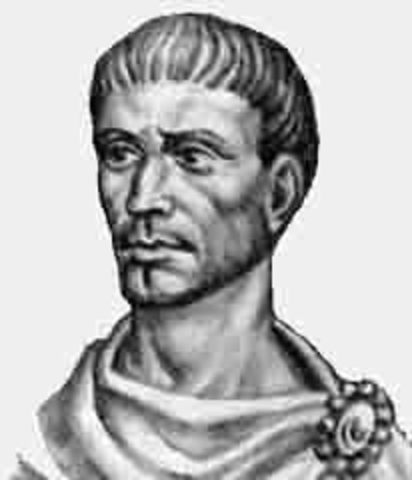
\includegraphics[width=\linewidth]{3}
                \caption{Диофант Александрийский}
                \label{fig:1}
            \end{subfigure}\hfill
            \begin{subfigure}[b]{.45\linewidth}
                \centering
                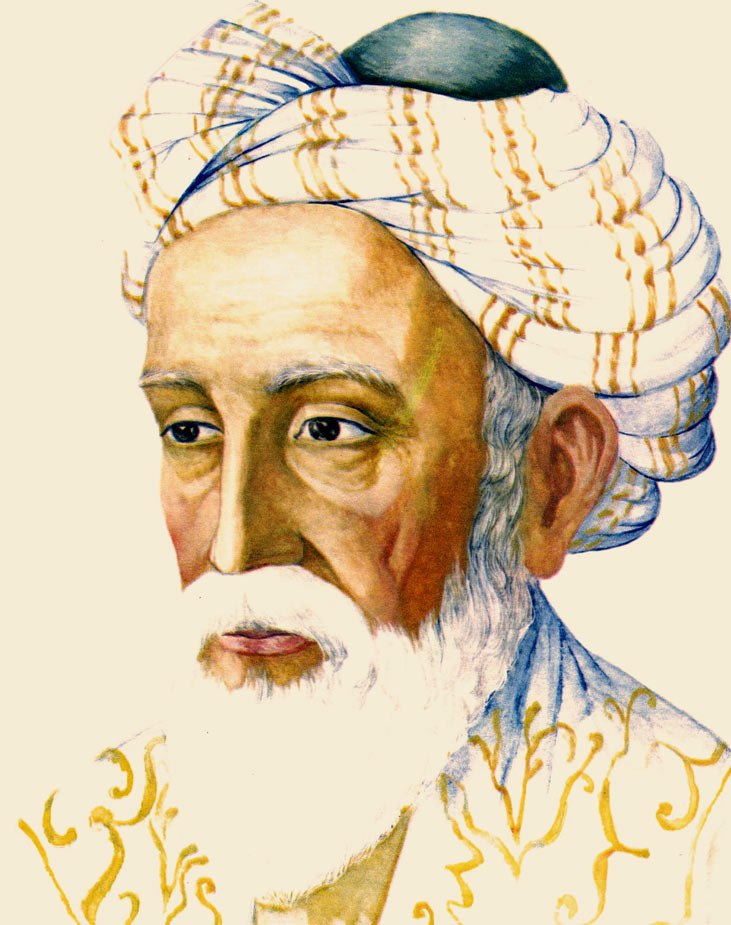
\includegraphics[width=\linewidth]{1}
                \caption{Омар Хайам}
                \label{fig:2}
            \end{subfigure}\\
            \caption{}
        \end{figure}
    }
    \frame{
	    \frametitle{Средние века}

        \begin{wrapfigure}{r}{0.4\textwidth}
            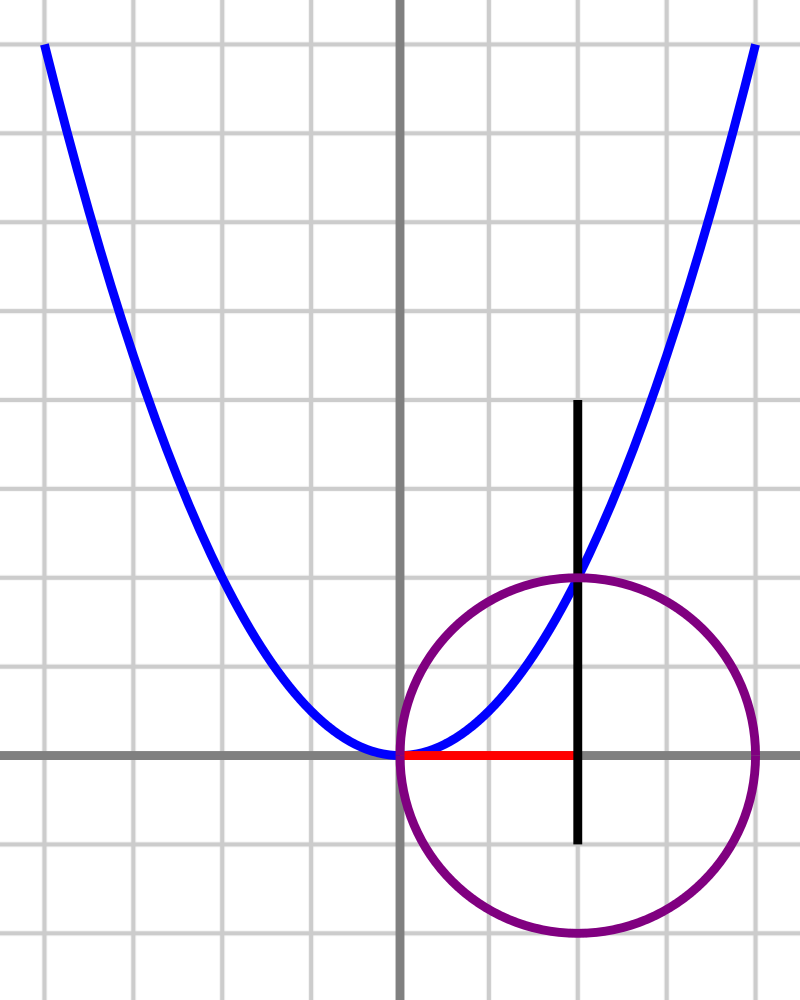
\includegraphics[width=2.5cm]{cubic.png}
            \caption{Геометрическое решение для случая $a=2,b=16$, дающее корень 2.}
            \label{fig2}
        \end{wrapfigure}

        Первые попытки решения кубических уравнений предпринимались ещё в средние века арабскими
        математиками. В частности, довольно интересный геометрический метод был предложен Омаром
        Хайямом. Для уравнения третьей степени вида $x^3+a^2x=b, \: b > 0$.
        Он строил окружность вида $y^2+x(x-\dfrac{b}{a^2})=0$, а затем искал её пересечение с
        параболой $y=\dfrac{x^2}{a}$.
	}
    \frame{
        \frametitle{Эпоха возрождения}
        Дальше, как хорошо известно, аналитический способ решения уравнений третьей степени был 
        найден итальянским математиком Сципионом дель Ферро в 16 веке. Однако обнародовано оно было
        только в книге Джероламо Кардано, вместе с общим методом решения алгебраического уравнения
        четвёртой степени, найденным учеником Кардано - Людовико Феррари. При этом вопрос о решении
        уравнений высших степеней оставался открытым. 
    }
    \frame{
        \frametitle{Дальнейшие исследования}
    }
\end{document}

